% !TEX TS-program = xelatex
% !BIB program = bibtex
% !TeX spellcheck = ru_RU

% About magic macros see also
% https://tex.stackexchange.com/questions/78101/

% По умолчанию используется шрифт 14 размера.
% Если Вы не влезаете в лимит страниц и нужен 12-й шрифт,
% то уберите опцию [14pt]
\documentclass[14pt, russian]{matmex-diploma-custom}

%%% Обязательные пакеты
%% Beamer
\usepackage{beamerthemesplit}
\usetheme{SPbGU}
\beamertemplatenavigationsymbolsempty
\usepackage{appendixnumberbeamer}

%% Локализация
\usepackage{fontspec}
\setmainfont{CMU Serif}
\setsansfont{CMU Sans Serif}
\setmonofont{CMU Typewriter Text}
%\setmonofont{Fira Code}[Contextuals=Alternate,Scale=0.9]
%\setmonofont{Inconsolata}
% \newfontfamily\cyrillicfont{CMU Serif}

\usepackage{polyglossia}
\setdefaultlanguage{russian}
\setotherlanguage{english}
\usepackage[autostyle]{csquotes} % Правильные кавычки в зависимости от языка

%% Графика
\usepackage{wrapfig} % Позволяет вставлять графику, обтекаемую текстом
\usepackage{pdfpages} % Позволяет вставлять многостраничные pdf документы в текст

%% Математика
\usepackage{amsmath, amsfonts, amssymb, amsthm, mathtools} % "Адекватная" работа с математикой в LaTeX

% Математические окружения с русским названием
\newtheorem{rutheorem}{Теорема}
\newtheorem{ruproof}{Доказательство}
\newtheorem{rudefinition}{Определение}
\newtheorem{rulemma}{Лемма}


%%% Дополнительные пакеты. Используются в презентации, но могут быть отключены при необходимости
\usepackage{tikz} % Мощный пакет для создание рисунков, однако может очень сильно замедлять компиляцию
\usetikzlibrary{decorations.pathreplacing,calc,shapes,positioning,tikzmark}

\usepackage{multirow} % Ячейка занимающая несколько строк в таблице

%% Пакеты для оформления алгоритмов на псевдокоде
\usepackage[noend]{algpseudocode}
\usepackage{algorithm}
\usepackage{algorithmicx}

\usepackage{fancyvrb}

%% Пакет для анимированных иллюстраций
\usepackage{animate}


\begin{document}
% TODO: Formatting
% !TeX spellcheck = ru_RU
% !TEX root = vkr.tex

%% Если что-то забыли, при компиляции будут ошибки Undefined control sequence \my@title@<что забыли>@ru
%% Если англоязычная титульная страница не нужна, то ее можно просто удалить.
\filltitle{ru}{
    %% Актуально только для курсовых/практик. ВКР защищаются не на кафедре а в ГЭК по направлению,
    %%   и к моменту защиты вы будете уже не в группе.
    chair              = {Кафедра системного программирования },
    group              = {23.Б08-мм},
    %
    %% Макрос filltitle ненавидит пустые строки, поэтому обязателен хотя бы символ комментария на строке
    %% Актуально всем.
    title = { 
       Улучшение производительности алгоритма достижимости с регулярными ограничениями на графическом ускорителе
    },
    %
    %% Здесь указывается тип работы. Возможные значения:
    %%   production - производственная практика;
    %%   coursework - отчёт по курсовой работе (ОБРАТИТЕ ВНИМАНИЕ, у техпрога и ПИ нет курсовых, только практики);
    %%   practice - отчёт по учебной практике;
    %%   prediploma - отчёт по преддипломной практике;
    %%   master - ВКР магистра;
    %%   bachelor - ВКР бакалавра.
    type               = {practice},
    %
    %% Здесь указывается вид работы. От вида работы зависят критерии оценивания.
    %%   solution - «Решение». Обучающемуся поручили найти способ решения проблемы в области разработки программного обеспечения или теоретической информатики с учётом набора ограничений.
    %%   experiment - «Эксперимент». Обучающемуся поручили изучить возможности, достоинства и недостатки новой технологии, платформы, языка и т. д. на примере какой-то задачи.
    %%   production - «Производственное задание». Автору поручили реализовать потенциально полезное программное обеспечение.
    %%   comparison - «Сравнение». Обучающемуся поручили сравнить несколько существующих продуктов и/или подходов.
    %%   theoretical - «Теоретическое исследование». Автору поручили доказать какое-то утверждение, исследовать свойства алгоритма и т.п., при этом не требуя написания кода.
    kind               = {solution},
    %
    author             = {Козенко Дмитрий Сергеевич},
    %
    %% Актуально только для ВКР. Указывается код и название направления подготовки. Типичные примеры:
    %%   02.03.03 \enquote{Математическое обеспечение и администрирование информационных систем}
    %%   02.04.03 \enquote{Математическое обеспечение и администрирование информационных систем}
    %%   09.03.04 \enquote{Программная инженерия}
    %%   09.04.04 \enquote{Программная инженерия}
    %% Те, что с 03 в середине --- бакалавриат, с 04 --- магистратура.
    specialty          = {02.03.03 \enquote{Математическое обеспечение и администрирование информационных систем}},
    %
    %% Актуально только для ВКР. Указывается шифр и название образовательной программы. Типичные примеры:
    %%   СВ.5162.2020 \enquote{Технологии программирования}
    %%   СВ.5080.2020 \enquote{Программная инженерия}
    %%   ВМ.5665.2022 \enquote{Математическое обеспечение и администрирование информационных систем}
    %%   ВМ.5666.2022 \enquote{Программная инженерия}
    %% Шифр и название программы можно посмотреть в учебном плане, по которому вы учитесь.
    %% СВ.* --- бакалавриат, ВМ.* --- магистратура. В конце --- год поступления (не обязательно ваш, если вы были в академе/вылетали).
    programme          = {СВ.5162.2020 \enquote{Технологии программирования}},
    %
    %% Актуально всем.
    %% Должно умещаться в одну строчку, допускается использование сокращений, но без переусердствования,
    %% короткая строка с большим количеством сокращений выглядит странно
    %supervisorPosition = {проф. кафeдры системного программирования, д.ф.-м.н.,}, % Терехов А. Н.
    %supervisorPosition = {ст. преподаватель кафедры ИАС, к.~ф.-м.~н. (если есть),}, % Смирнов К. К.
    supervisorPosition = {доцент кафедры системного программирования, к.~ф.-м.~н.,},
    supervisor         = {Григорьев С. В.},
    %
    %% Актуально только для практик и курсовых. Если консультанта нет или он совпадает с научником, закомментировать или удалить вовсе.
    % consultantPosition = {должность, ООО \enquote{Место работы}, степень  (если есть),},
    % consultant         = {Консультант~К.~К.},
    %
    %% Актуально только для ВКР.
    reviewerPosition   = {должность, ООО \enquote{Место работы}, степень (если есть),},
    reviewer           = {Рецензент~Р.~Р.},
}

% Английский титульник нужен только для ВКР, остальные виды работ могут его смело игнорировать.
\filltitle{en}{
    chair              = {Advisor's chair},
    group              = {ХХ.BХХ-mm},
    title              = {Template for SPbU qualification works},
    type               = {bachelor},
    author             = {FirstName Surname},
    %
    %% Possible choices:
    %%   02.03.03 \foreignquote{english}{Software and Administration of Information Systems}
    %%   02.04.03 \foreignquote{english}{Software and Administration of Information Systems}
    %%   09.03.04 \foreignquote{english}{Software Engineering}
    %%   09.04.04 \foreignquote{english}{Software Engineering}
    %% Те, что с 03 в середине --- бакалавриат, с 04 --- магистратура.
    specialty          = {02.03.03 \foreignquote{english}{Software and Administration of Information Systems}},
    %
    %% Possible choices:
    %%   СВ.5162.2020 \foreignquote{english}{Programming Technologies}
    %%   СВ.5080.2020 \foreignquote{english}{Software Engineering}
    %%   ВМ.5665.2022 \foreignquote{english}{Software and Administration of Information Systems}
    %%   ВМ.5666.2022 \foreignquote{english}{Software Engineering}
    programme          = {СВ.5162.2020 \foreignquote{english}{Programming Technologies}},
    %
    %% Note that common title translations are:
    %%   кандидат наук --- C.Sc. (NOT Ph.D.)
    %%   доктор ... наук --- Sc.D.
    %%   доцент --- docent (NOT assistant/associate prof.)
    %%   профессор --- prof.
    supervisorPosition = {Sc.D, prof.},
    supervisor         = {S.S. Supervisor},
    %
    consultantPosition = {position at \foreignquote{english}{Company}, degree if present},
    consultant         = {C.C. Consultant},
    %
    reviewerPosition   = {position at \foreignquote{english}{Company}, degree if present},
    reviewer           = {R.R. Reviewer},
}

\maketitle
\setcounter{tocdepth}{2}
\tableofcontents

% !TeX spellcheck = ru_RU
% !TEX root = vkr.tex

\section*{Введение}
\thispagestyle{withCompileDate}

В последние годы графовые базы данных набирают все большую популярность:
они используются в алгоритмах для социальных сетей~\cite{SocNets}, в создании баз 
знаний~\cite{Knowledge}, в медицине~\cite{ChemRecEngine}. Хотя они и имеют ряд ограничений
и недостатков, во многих задачах они показывают себя намного лучше, чем реляционные базы
данных~\cite{GraphDatabases}.
В них данные представляются как граф с метками на вершинах (которые представляют объекты)
и на ребрах (которые представляют отношения между объектами). Одна из естественных задач,
возникающая при работе с такими базами данных, --- нахождение всех объектов, связанными
определенными отношениями с заданным. Для решения ее надо искать в графе пути с
определенными ограничениями. Если рассматривать всевозможные метки на ребрах как алфавит,
а путь в графе как слова, то ограничения можно проклассифицировать формальными языками~\cite{FormPathReg}.
Бyдем рассматривать регулярные языки над этим алфавитом и использовать регулярные ограничения,
а точнее их расширение –-- двухсторонние регулярные ограничения, позволяющие
ходить по ребрам в обратном направлении. Запросы с двухсторонними регулярными
ограничениями были реализованы в языке запросов
к данным SPARQL, и добавлены в ISO стандарт языков запросов к графам в ISO 
39075:2024\footnote{Стандарт ISO/IEC 39075:2024: \url{https://www.iso.org/standard/76120.html} (Дата посещения: 09.11.2024)}.

В реализациях алгоритмов для решения этой задачи активно используются представление графов в
виде разреженных матриц смежности, например в графовых базах данных MilleniumDB~\cite{MilleniumDB} и FalcorDB\footnote{Документация FalcorDB: \url{https://docs.falkordb.com/} (Дата посещения: 08.01.2025)}. 
Так же есть алгоритмы, представленные в работax~\cite{sparse-rpq-1} и~\cite{OldRpqVkr}, основанные на операциях линейной алгебры.

Операции линейной алгебры отлично ложатся на огромную вычислительную мощность видеокарт,
и хочется использовать этот потенциал для улучшения времени работы алгоритма. Есть
различные библиотеки, позволяющие работать с булевой линейной алгеброй на 
GPU: Spla~\cite{Spla}, Cusp\footnote{Репозитория Cusp на GitHub: \url{https://github.com/cusplibrary/cusplibrary} (Дата посещения: 08.01.2025)}, cuBool~\cite{CuBool}.
Библиотека cuBool~\cite{CuBool} в тестах\footnote{Тесты производительности cuBool: \url{
https://github.com/SparseLinearAlgebra/cuBool?tab=readme-ov-file\#performance} (Дата посещения: 08.01.2025)}
производительности показывает себя лучше всего, но она не поддерживает последнюю
версию вычислительного API CUDA и в ней нет некоторой функциональности,
необходимой для реализации алгоритма.

В данной работе будет представлена адаптация алгоритма достижимости с регулярными 
ограничениями для GPGPU вычислений и его 
реализация на вычислительном API CUDA для графических ускорителей.
% !TeX spellcheck = ru_RU
% !TEX root = vkr.tex

\section{Постановка задачи}
\label{sec:task}

Целью работы является адаптация алгоритма достижимости с регулярными ограничениями
для GPGPU вычислений и его перенос на видеокарту с помощью библиотеки cuBool \cite{CuBool}.
Для достижения поставленной выше цели необходимо выполнить следующие задачи.
\begin{enumerate}
    \item Обновить библиотеку cuBool для поддержки последней версии CUDA.
    \item Реализовать в cuBool недостающие для алгоритма операции с булевыми
          матрицами.
    \item Реализовать алгоритм, используя обновленную библиотеку.
    \item Провести эксперименты: найти узкие места в алгоритме и уменьшить среднее
          время исполнения, сравнить время работы
          реализации алгоритма на GPU с его реализацией на CPU и проанализировать результаты.
\end{enumerate}

% !TeX spellcheck = ru_RU
% !TEX root = vkr.tex

\section{Обзор}
\label{sec:relatedworks}

% \subsection{Выбранная реализация алгоритма}

У алгоритма достижимости с регулярными ограничениями есть довольно много реализаций, из популярных можно назвать реализации в больших графовых базах данных с открытым кодом
MilleniumDB\footnote{Реализация RPQ в MilleniumDB: \url{https://github.com/MillenniumDB/MillenniumDB/tree/main/src/query/executor/binding_iter/paths/all_shortest_simple} (Дата посещения: 08.01.2025)} и
FalcorDB\footnote{Реализация RPQ в FalcorDB: \url{https://github.com/FalkorDB/FalkorDB/blob/master/src/algorithms/all_shortest_paths.c} (Дата посещения: 08.01.2025)}.

Но для реализации на GPU был выбран алгоритм, предложенный Георгием Беляниным в работе \cite{OldRpqVkr}. Реализация этого алгоритма на CPU от автора работы представлена в GitHub репозитории\footnote{Реализация алгоритма RPQ: \url{https://github.com/SparseLinearAlgebra/LAGraph/tree/2-rpq} (Дата посещения: 08.01.2025)}. Она реализованна на базе библиотеки линейной алгебры для разреженных матриц SuiteSparse ~\cite{SuiteSparse} в форке репозитория LaGraph, где собраны алгоритмы на базе этой библиотеки.

Причины, по которым была выбрана именно она, перечислены ниже.
\begin{itemize}
    \item Она основана на операциях булевой линейной алгебры и использует большие разреженные матрицы, а вычисления этих операций отлично подходят для огромной параллельной вычислительной мощности видеокарт.
    \item Есть поддержка двухсторонниx запросов.
    \item В библиотеке SuiteParse ведется разработка поддержки вычислений на GPU, так что потенциально именно эта реализация может стать главным конкурентом по производительности.
    \item В работе~\cite{rpq-article-cool} есть тесты производительности, которые говорят о том, что алгоритм работает быстрее своих конкурентов.
\end{itemize}

В работе можно найти следующий псевдокод алгоритма (\ref{AlgoCode}).

\begin{algorithm}[H]
    \caption{Алгоритм достижимости в графе с регулярными ограничениями на основе поиска в ширину, выраженного с помощью операций матричного умножения}
    \label{AlgoCode}
    \begin{algorithmic}[1]
        \Procedure{BFSBasedRPQ}{$D = \langle Q, q_S, Q_F, \delta, \Sigma \rangle,G=\langle V, E, L \rangle, V_{src}$}
            \State $\mathcal{D}^a\gets $ Матрица смежности ДКА для символа $a$
            \State $\mathcal{G}^a\gets $ Матрица смежности графа для символа $a$
            \State $\mathcal{F}\gets $ Вектор финальных состояний автомата $D$
            \State $M\gets$ Матрица $|Q| \times |V|$ \Comment Матрица обхода
            \State $P\gets$ Матрица $|Q| \times |V|$ \Comment Матрица с посещёнными состояниями
            \State $M'\gets$ Матрица $|Q| \times |V|$ с вершинами из $V_{src}$, соответствующими $q_S$

            \While{$M'$ ненулевая}{}
                \State $M\gets M'$
                \State $M'\gets$ Пустая матрица
                \ForAll{$a\in (\Sigma \cap L)$}
                    \If{$a$ начинается не с $\^{}$}
                        \State $M'\gets M' + (\mathcal{D}^a)^T \times (M \times \langle \neg P \rangle \mathcal{G}^a)$ \Comment{Умножение с маской}
                    \Else
                        \State $M'\gets M' + (\mathcal{D}^a)^T \times (M \times \langle \neg P \rangle (\mathcal{G}^a)^T)$
                    \EndIf
                \EndFor
                \State $P\gets P + M'$ \Comment{Аккумулирование достигнутых состояний}
                \State $\mathcal{P}\gets \mathcal{P} + \mathcal{F} \times M'$ \Comment{Поиск финальных состояний}
            \EndWhile
            \State \textbf{return} $\mathcal{P}$
        \EndProcedure
    \end{algorithmic}
    \label{final-algo}
\end{algorithm}

Список входных параметров перечислен ниже.
\begin{itemize}
    \item Конечный автомат, построенный по регулярному ограничению (существуют алгоритмы преобразования), состоящий из графа переходов $Q$, начальных ($q_S$) и конечных ($Q_F$) состояний, а так же алфавита $\delta$ и языка $\Sigma$ на котором построено регулярное ограничение. 
    \item Граф, состоящий из множества вершин $V$, множества ребер с метками $E$ и множества допустимых меток $L$.
    \item Начальные вершины графа --- $V_{src}$.
\end{itemize}

Граф декомпозируются по меткам (для каждой метки выделяется граф, состоящий из тех же вершин, что и начальный граф, но из ребер начального графа берутся только ребра с этой меткой), и создаётся множество матриц смежности для каждого получившегося графa $\mathcal{D}^a$. Такая же операция применяется и к графу конечного автомата $\mathcal{G}$.

Далее создаются матрицы, которые будут обновляться каждый шаг алгоритма и хранить текущее состояние: все достижимые вершины на данном шаге алгоритма. Это матрицы обхода $M$ и $M'$, одна пустая (так как на первом же шаге цикла в нее будет записано другое значение), а вторая заполняется следующим образом: для каждого начального состояния конечного автомата все начальные вершины графа помечаются достижимыми.
Так же создается матрица всех посещенных состояний $P$, чтобы в дальнейшем избежать лишних итераций цикла алгоритма.

Основная часть алгоритма --- это обход поиском в ширину, который происходит с использованием умножения матриц. Он продолжается, пока матрица обхода c предыдущего шага $M'$ ненулевая. Каждый шаг матрица обхода с предыдущего шага сохраняется, матрица обхода текущего шага заполняется нулями.

На каждом шагу обхода алгоритм проходит по всем исходящим из вершин, достигнутых на предыдущем шаге, ребрам для каждой метки, одновременно обходится и конечный автомат. Это происходит следующим образом: к матрице обхода состояния $M'$ для каждой метки $a$ аккумулируются состояния, получающиеся из вершин прошлого состояния, которые еще не были посещены (это достигается при помощи умножения на маску посещенных состояний $P$), проходя по ребру, если оно есть и в графе (умножение на $\mathcal{G}^a$), и в графе конечного автомата (умножаем на $\mathcal{D}^a$ на результат прохода по ребру графа). Если по ребру требуется пройти в обратную сторону, то используется транспонированную матрицу графа $(\mathcal{G}^a)^T$ (доказательство корректности операции можно найти в работе в пункте 3.1). 

После этого мы обновляем матрицу посещенных состояний $P$ и вектор финальных состояний $\mathcal{P}$ (дописываем в него, в какой вершине мы достигли какого-то финального состояния конечного автомата).  

Результатом алгоритма является вектор финальных состояний $\mathcal{P}$.

\subsection{Выбор библиотеки булевой линейной алгебры для GPU}

Проанализировав алгоритм, можно составить список необходимых операций, который должна поддерживать искомая библиотека булевой линейной алгебры для GPU. Все перечисленные ниже операции подразумевают умножение и сложение над булевым полукольцом.

\textit{Инвертированной матрицей} для матрицы $A$ называется матрица такого же размера, у которой на месте 1 у матрицы $A$ стоит 0, а на месте 0 --- 1. 

\begin{enumerate}
    \item Перемножение булевых матриц.
    \item Возможность транспонировать и сохранить матрицу.
    \item Поэлементное умножение на инвертированную матрицу.
    \item Поэлементное сложение матриц.
    \item Операция получения количества ненулевых элементов.
    \item Умножение вектора на матрицу.
\end{enumerate}

Также очень важным фактором является формат хранения матриц: ожидается, что алгоритм должен уметь работать с графами, в которых порядка $10^8$ вершин, и если хранить матрицу в виде двумерного массива, то это займет невозможное в нынешнее время количество памяти. 
При этом в алгоритме матрицы преимущественно разреженные, так что рассматривались библиотеки, использующие оптимальные структуры данных для хранения разреженных матриц.

Были найдены следующие библиотеки, подходящие по данному критерию: Spla~\cite{Spla}, Cusp\footnote{Репозитория Cusp на GitHub: \url{https://github.com/cusplibrary/cusplibrary} (Дата посещения: 08.01.2025)}, cuBool~\cite{CuBool}.
Сравнивая их по скорости работы и легкости интеграции и отладки, была выбрана библиотека cuBool по следующим причинам.

\begin{itemize}
    \item Скорость работы\footnote{Тесты производительности cuBool: \url{
https://github.com/SparseLinearAlgebra/cuBool?tab=readme-ov-file\#performance} (Дата посещения: 08.01.2025)}. Это является ключевым требованием, так как хочется добиться максимальной производительности и обрабатывать графы из реального мира.
    \item Её легковесность и сравнительная простота: читабельность кода и возможность быстро разобраться в нем чрезвычайно важны при разработке, так как для достижения максимальной производительность придется отлаживать даже функции внутри самой библиотеки, и необходимо разбираться в том, как они работают. Также библиотека почти не использует сложные API для вычислений на видеокарте, вместо это в ней используется библиотека thrust\footnote{Библиотека thrust: \url{https://developer.nvidia.com/thrust} (Дата посещения: 08.01.2025)}, которая хорошо задокументирована.
    \item Возможность обновлять ее и дописывать свой код.
\end{itemize}

\subsection{Библиотека cuBool}
В этом разделе будет более подробно рассмотрена библиотека cuBool, ее возможности и недостатки.

В cuBool представлены почти все операции булевой линейной алгебры для векторов и матриц. Для матриц это транспонирование, сложение, умножение, как обычное, так и поэлементное, операция взятия столбца или строки как вектор, сложение всех строк, а также произведение Кронекера. Что очень важно, есть операция получения количества ненулевых элементов, и при этом она работает за $O(1)$. Для векторов же это сложение и умножение как вектора на матрицу, так и матрицы на вектор.

Но при наличии большого набора операций нет одной, необходимой для алгоритма: поэлементного умножения на инвертированную матрицу.

Все матрицы в cuBool разреженные, и используется следующий формат хранения: для каждой матрицы хранится множество пар индексов с ненулевыми значениями.  

Для реализации данных операций данная библиотека использует вычислительное API CUDA\footnote{API CUDA: \url{https://developer.nvidia.com/cuda-toolkit} (Дата посещения: 08.01.2025)} от Nvidia, а точнее говоря библиотеку thrust, написанную на CUDA самими разработчиками. Полная и доступная документация thrust\footnote{Документация thrust: \url{https://nvidia.github.io/cccl/thrust/} (Дата посещения: 08.01.2025)} делает разработку на ней быстрой и приятной, а код становится легко читабельным.

В cuBool есть поддержка операций, выполняемых на CPU без использования параллельных вычислений, что конечно не дает желаемой производительности, но позволяет запускаться на платформах, на которых нет графического ускорителя.

Также в cuBool есть удобная система логгирования, сильно облегчающая отладку, а также слежение за выделенной памятью, что помогает избежать её утечек.

Еще одной проблемой стало отсутствие поддержки в последние годы: последний раз cuBool был собран компилятором gcc версии 8 и протестирован на CUDA версии 10.1 (версия датируется 28 июля 2019 года). При тестировании на компьютере с последней версией CUDA 12.6 (от 14 августа 2024 года) и gcc 14.2 возникло большое количество ошибок компиляции.

\subsection{Поэлементное умножение разреженных булевых матриц}

Так как в cuBool не хватает реализации умножения на инвертированную матрицу, необходимо изучить, как реализовать эту операцию, учитывая формат хранения разреженных матриц в cuBool.

Дан простой пример поэлементного умножения матриц.

\begin{align*}
\begin{pmatrix}
  1 & 0 & 0 & 1  \\
  1 & 0 & 0 & 0  \\
  0 & 0 & 1 & 1  \\
  1 & 0 & 1 & 0  \\
\end{pmatrix}
* 
\begin{pmatrix}
  1 & 0 & 0 & 0  \\
  0 & 1 & 1 & 0  \\
  1 & 0 & 0 & 0  \\
  1 & 0 & 1 & 1  \\
\end{pmatrix}
=
\begin{pmatrix}
  1 & 0 & 0 & 0  \\
  0 & 0 & 0 & 0  \\
  0 & 0 & 0 & 0  \\
  1 & 0 & 1 & 0  \\
\end{pmatrix}
\end{align*}

Пусть $C = A * B$. Для каждого элемента итоговой матрицы довольно легко понять, какое значение у него будет. Он равен единице тогда и только тогда, когда у каждой перемножаемой матрицы соответствующие элементы тоже равны единицам.
$$
C_{ij} = 1
\Longleftrightarrow
\begin{cases}
    A_{ij} = 1 \\
    B_{ij} = 1
\end{cases}
$$

Один из оптимальных по памяти форматов представления разреженных матриц это множество пар индексов, в которых элементы отличны от 0. И чтобы вычислить результат поэлементного умножения надо узнать, все пары индексов, которые есть в обоих исходных матрицах, то есть нужно пересечь множества индексов с ненулевыми элементам матриц.

Теперь легко можно вывести правило для поэлементного умножения на инвертированную матрицу.
Все единицу у матрицы $B$ переходят в нули, а нули -- в единицу.
$$
C_{ij} = 1
\Longleftrightarrow
\begin{cases}
    A_{ij} = 1 \\
    B_{ij} = 0
\end{cases}
\Longleftrightarrow
\begin{cases}
    A_{ij} = 1 \\
    B_{ij} \ne 1
\end{cases}
$$

ля получения итоговой матрицы нам нужно узнать все индексы, в которых у элемента первой матрицы значение единица, а у элемента второй матрицы значение 0. Для получения этого множества индексов надо вычесть из множества индексов с ненулевыми элементами первой матрицы множество индексов с ненулевыми элементами второй матрицы.

% !TeX spellcheck = ru_RU
% !TEX root = vkr.tex

\section{Анализ производительности и улучшения алгоритма}

В начале работы был воспроизведен эксперимент из предыдущей работы~\cite{PrevWork} --- проведены замеры производительности реализаций на GPU и CPU на наборе данных Wikidata\footnote{База знаний \textsc{WikiData}: \href{https://www.wikidata.org/wiki/Wikidata:Database_download}{https://www.wikidata.org/wiki/Wikidata:Database\_download} (Дата доступа: 19.06.2025)} \cite{wikidata}. Время выполнения всех первых 520 запросов следующее: для CPU --- 98.3 секунды, для GPU --- 273.3 секунды.

Далее к реализации на GPU был применён анализатор производительности Intel Vtune\footnote{Анализатор vtune: \url{https://www.intel.com/content/www/us/en/developer/tools/oneapi/vtune-profiler.html} (Дата доступа: 19.06.2025)}, был составлен FlameGraph. Распределение времени работы по функциям предоставлено в таблице \ref{tab:FlameGraph1}.      

\begin{table}[ht]
\centering
\caption{Распределение времени работы внутри алгоритма}
\label{tab:FlameGraph1}
\begin{tabular}{|l|l|l|}
\hline
Функция cuBool & Время работы, сек & Часть в \% \\
\hline
\verb|cuBool_Matrix_EWiseAdd| & 164.2 & 60.1\% \\
\verb|cuBool_MxM| & 70.7 & 25.9\% \\
\verb|cuBool_Matrix_Transpose| & 30.5 & 11.2\% \\
\verb|cuBool_Matrix_EWiseMulInverted| & 6.0 & 2.2\% \\
\verb|cuBool_Matrix_Free| & 1.7 & 0.6\% \\
\hline
\end{tabular}
\end{table}

То, что функция сложения матриц занимает больше всего времени, очень необычно. Если посмотреть на псевдокод алгоритма \ref{AlgoCode}, то можно заметить, что операция сложения применяется не чаще операции поэлементного умножения на инвертированную матрицу, а асимптотически операции очень похожи, это видно из сравнения пункта \ref{MatrixAddSection} и пункта 3.3 из работы~\cite{PrevWork}. Но функция сложения занимает в разы больше времени относительно функции поэлементного умножения на инвертированную матрицу.

Была изучена реализация функции сложения матриц\footnote{\href{https://github.com/SparseLinearAlgebra/cuBool/blob/ab425e17000af8763e7b2cdf020589f8b2db371d/cubool/sources/cuda/kernels/spmerge.cuh#L36}{Код} предыдущей реализации сложения матриц в cuBool (Дата доступа: 19.06.2025)} в cuBool. Было обнаружено, что она использует библиотеку nsparse~\cite{Nsparse}. Для проверки гипотезы, что эта реализация не дает достаточной производительности, функция сложения была реализована аналогично функции умножения на инвертированную матрицу. Для сохранения старой функциональности была добавлена опция для выбора реализации функции сложения --- \verb|CUBOOL_USE_NSPARSE_MERGE_FUNCTOR|.

При применении vtune для версии с новой функцией сложения матриц, видно значительное ускорение в 2.34 раза, теперь время выполнения всех запросов составляет 116.6 секунд, а время работы самой функции сложения матриц сократилось с 164.2 секунд до 10.5, то есть ускорение в 15.6 раз.

Так же была обнаружена ошибка в файле CmakeLists.txt библиотеки cuBool (Листинг \ref{IncorrectCompileOptions}) --- перепутаны флаги оптимизаций для компилятора в конфигурациях Debug и Release. В Debug используются оптимизации компилятора, а в Release --- нет. Было убрано явное выставление флагов, так как хорошей практикой при написании CmakeLists считается не выставлять явно флаги компиляции, если нет необходимости.

% Листинг \ref{CmakeOption})
\begin{listing}
    \caption{Ошибочное выставление флагов компиляции}
    \begin{minted}[fontsize=\small]{Cmake}
target_compile_options(cubool PRIVATE $<$<AND:$<CONFIG:Debug>,
                                        $<COMPILE_LANGUAGE:CXX>>: -O2>)
target_compile_options(cubool PRIVATE $<$<AND:$<CONFIG:Release>,
                                        $<COMPILE_LANGUAGE:CXX>>: -O0>)
  \end{minted}
\label{IncorrectCompileOptions}
\end{listing}


Это изменение не повлияло на время выполнения запросов (так как эти опции не относятся к кернелам CUDA, в которых происходят сами вычисления), зато сильно повлияло на время загрузки запросов: функция преобразования матриц в формат CSR \verb|cuBool_Matrix_Build| стала работать в 8.3 раз быстрее --- вместо 5686.4 секунд 686.3 секунд.

Так же после анализа времени работы алгоритма на CPU было обнаружено, что транспонирование матриц не занимает времени, в то время как в реализации для GPU оно занимало около 25\%. Было замечено, что в бенчмарке для CPU транспонированные матрицы уже передаются в алгоритм. После этого была добавлена такая возможность и в бенчмарк для реализации для GPU.

\subsection{Организация репозитории cuBoolGraph}

Была организована GitHub репозиторий cuBoolGraph\footnote{Репозиторий cuBoolGraph: \url{https://github.com/SparseLinearAlgebra/cuBoolGraph} (Дата доступа: 19.06.2025)} в ветке \texttt{add-rpq}. Была выбрана следующая структура файлов (Листинг \ref{cuBoolGraphFiles}).

\begin{listing}[H]
    \caption{Структура файлов cuBoolGraph}
    \label{cuBoolGraphFiles}
    
    \begin{minted}[]{shell} 
cuBoolGraph
├── deps
│   ├── cuBool
│   ├── fast_matrix_market
│   └── googletest
├── include
├── src
└── tests
    └── test_data
   \end{minted}
\end{listing}

В директории \verb|src| находятся исходные файлы алгоритмов, в \verb|include| --- их заголовочные файлы. Также есть директория с тестами \verb|tests|. В директории \verb|deps| лежат внешние зависимости. Это, естественно, библиотека \verb|cuBool|, а также зависимости для тестирования --- \verb|googletests|\footnote{GitHub репозиторий googletests: \url{https://github.com/google/googletest} (Дата доступа: 19.06.2025)} и \verb|fast_matrix_market|\footnote{GitHub репозиторий \texttt{fast\_matrix\_market}: \url{https://github.com/alugowski/fast_matrix_market} (Дата доступа: 19.06.2025)} для загрузки матриц в формате matrix market. Все зависимости присоединяются к библиотеке при помощи \verb|git submodule|. Также был настроен CI, в котором запускаются тесты.


% !TeX spellcheck = ru_RU

\section{Эксперимент}

После реализации алгоритма было необходимо протестировать его работоспособность на данных из реального мира и сравнить его производительность с реализацией на CPU, чтобы понять, что дал перенос алгоритма для вычислений на видеокарте.

В качестве данных была выбрана база знаний \textsc{Wikidata}\footnote{База знаний \textsc{WikiData}: \href{https://www.wikidata.org/wiki/Wikidata:Database_download}{https://www.wikidata.org/wiki/Wikidata:Database\_download} (Дата доступа 11.12.24)} \cite{wikidata}, на которой тестировалась производительность реализации на CPU в работе ~\cite{OldRpqVkr}, так как это один из самых разнообразных и больших графов доступных публично и вместе с ним доступны наборы реальных регулярных запросов. Код\footnote{Код для теста производительности алгоритма: \url{https://github.com/georgiy-belyanin/RPQ-bench} (Дата посещения: 08.01.2025)} для теста производительности выложен автором алгоритма на GitHub.

\subsection{Условия эксперимента}
Эксперименты проводились на тестовом стенде со следующей конфигурацией.
\begin{itemize}
    \item \textbf{CPU}: Intel i5-10400f, 6 физических, 12 логических ядер, максимальная частота 4.3 GHz
    \item \textbf{GPU}: Nvidia RTX 3050, 8 Gb VRAM, 1552 MHz
    \item \textbf{RAM}: 16 Gb, 3200 MHz, DDR4
    \item \textbf{OS}: Ubuntu 24.04
    \item \textbf{Компиляторы}: nvcc 12.6, gcc 14.2
\end{itemize}
Измерялось только время работы алгоритма, загрузка входных данных в оперативную память и видеопамять не учитывалась.

Тестирование проводилось на 520 запросах, среди которых встречаются двусторонние. Размеры графа порядка $10^8$, что позволяет протестировать алгоритм на графe большого размера.

Погрешности измерения не указаны, так как они достаточно малы.
Для каждого алгоритма все запросы были проведены по 10 раз, и стандартное отклонение только у 1 запроса для GPU превысило 1\%, для измерений на CPU у 6 запросов, но ни одно стандартное отклонение не превысило 8\%.

\begin{figure}[H]
    \centering
    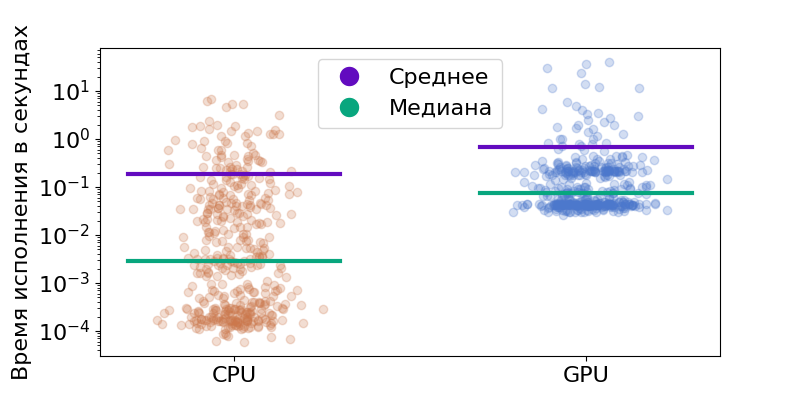
\includegraphics[scale = 0.85]{Cloud.png}
    \caption{Облако распределения времени исполнения запросов}
    \label{GraphicFull}
\end{figure}

\begin{figure}[H]
    \centering
    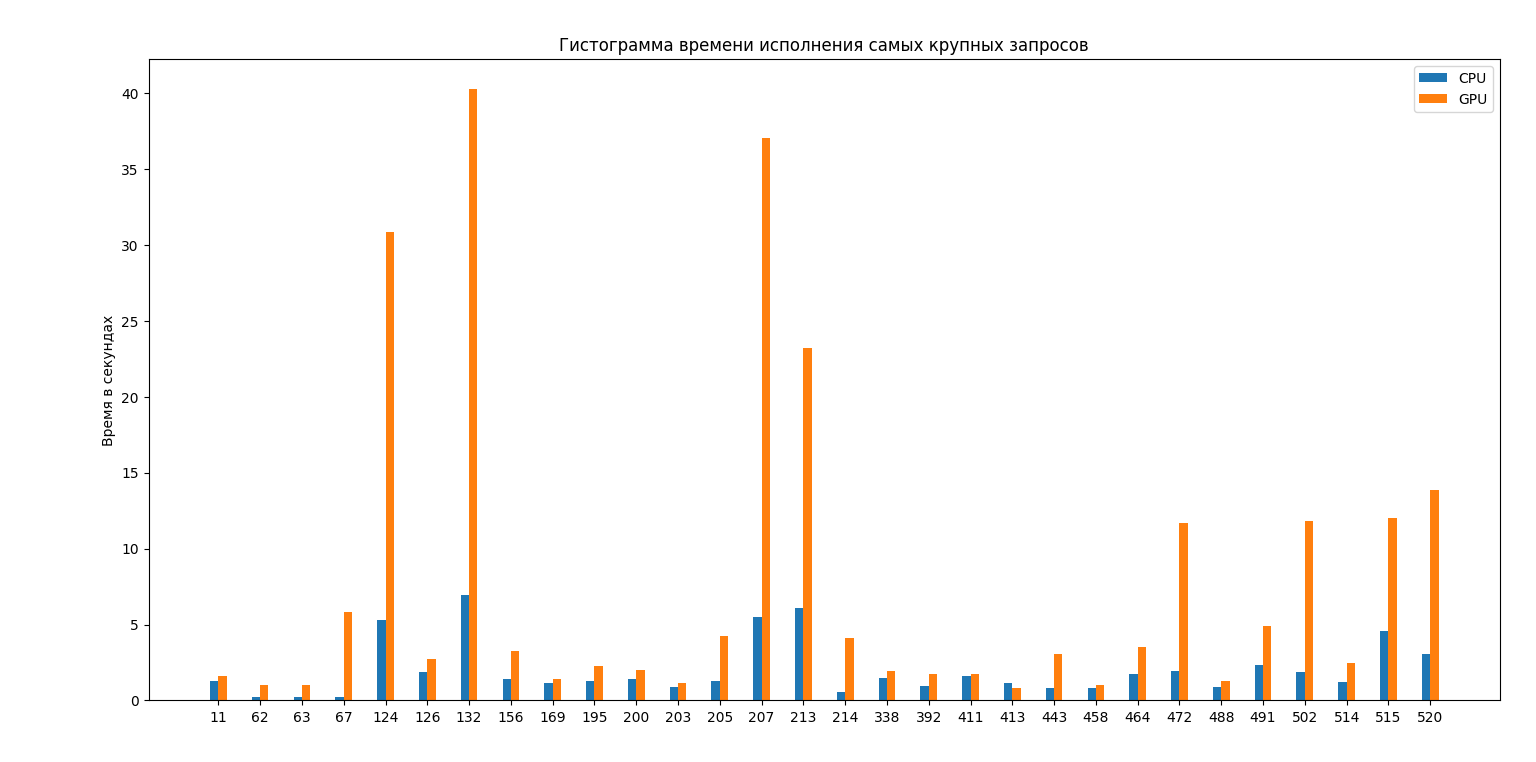
\includegraphics[scale = 0.42]{HistBig.png}
    \caption{Гистограмма времени исполнения самых крупных запросов (занявших более 1 секунды)}
    \label{GraphicBig}
\end{figure}

\newpage

Было построено облако распределения времени работы (Рис. \ref{GraphicFull}) реализаций на CPU и GPU на разных запросах. Заметно, что даже маленькие запросы реализация на GPU исполняет с некоторой задержкой. Так же была построена гистограмма для выборки самых крупных запросов, в которых время работы одной из реализации больше 1 секунды (Рис. \ref{GraphicBig}). Можно заметить, что есть отдельные запросы, на которых реализация на GPU работает намного хуже реализации на CPU. В дальнейшем следует подробнее изучить эти запросы и выявить закономерности.

Было посчитано среднее замедление, оно равняется 3.59. Этот показатель говорит о том, что текущая реализация алгоритма на GPU проигрывает реализации на CPU. Но есть и 20 запросов, на которых реализация на GPU выигрывает.

Для дальнейших исследований для каждого запроса было посчитано ускорение, взята медиана и посчитано среднее арифметическое: среднее арифметическое равняется 0.232, а медиана 0.0379. То, что медиана ускорений примерно в 8 раз меньше среднего показывает, что запросы делятся на те, на которых реализация на GPU проигрывает сильно, и те, на которых проигрыш не так заметен. Это также можно увидеть на графике (Рис. \ref{GraphicFull}).

Также были проанализированны лучшие и худшие показатели ускорения: взято среднее арифметическое по 5 лучшим (Таблица \ref{Best5Queries}) и 5 худшим (Таблица \ref{Worst5Queries}). У лучших этот показатель равняется 1.584, что говорит о том, что есть запросы, на которых реализация на GPU показывает себя значительно лучше реализации на CPU. Худший показатель же крайне мал: 0.000603. Это говорит о том, что есть отдельный тип запросов, с которыми реализация на GPU крайне плохо работает. Можно заметить, что время работы у алгоритма на CPU крайне мало, и возможно такая большая разница из-за того, что сама работа с GPU занимает всегда какое-то время, которое незначительно в более крупных запросах, но в таких малых превышает время вычислений.

\begin{table}[]
\centering
    \begin{tabular}{|c|c|c|c|}
    \hline
         Номер запроса & Время GPU & Время CPU & Ускорение \\
    \hline
        353 & 0.182 & 0.263 & 1.444 \\
        421 & 0.294 & 0.441 & 1.501 \\
        416 & 0.431 & 0.704 & 1.633 \\
        346 & 0.277 & 0.46  & 1.658 \\
        311 & 0.179 & 0.3   & 1.682 \\
    \hline
    \end{tabular}
    \caption{5 лучших запросов}
    \label{Best5Queries}
\end{table}

\begin{table}[]
\centering
    \begin{tabular}{|c|c|c|c|}
    \hline
         Номер запроса & Время GPU & Время CPU & Ускорение \\
    \hline
        429 & 0.170 & 0.000081 & 0.000476 \\
        511 & 0.200 & 0.000111 & 0.000553 \\
        484 & 0.202 & 0.000127 & 0.000627 \\
        433 & 0.175 & 0.000118 & 0.000671 \\
        442 & 0.174 & 0.000119 & 0.000683 \\
    \hline
    \end{tabular}
    \caption{5 худших запросов}
    \label{Worst5Queries}
\end{table}


Результаты эксперимента показали, что реализация алгоритма на GPU хорошо справляется с данными из реального мира, но при этом проигрывает в производительности реализации на CPU. Изучение среднего замедления показало, что среднее время исполнения запроса того же порядка, что и время исполнения запроса на CPU, а на некоторых запросах реализация на GPU показала себя даже лучше, следовательно реализацию на GPU можно использовать для распределения нагрузки на графические ускорители при многочисленных запросах. Анализ типов запросов, на которых реализация на GPU показывает себя лучше реализации на CPU или наоборот сильно ей проигрывает не был проведен, он планируется в дальнейших исследованиях алгоритма.  


% !TeX spellcheck = ru_RU
% !TEX root = vkr.tex

\section{Заключение}

В ходе работы над реализацией алгоритма достижимости с регулярными ограничениями на графическом ускорителе были достигнуты следующие результаты.

\begin{itemize}
    \item Библиотека cuBool была обновлена до последней версии CUDA 12.6.
    \item В cuBool реализована операция поэлементного умножения на инвертированную матрицу.
    \item При помощи обновленной версии cuBool алгоритм достижимости с регулярными ограничениями был реализован для запуска на GPU.
    \item Был проведен эксперимент, который показал, что текущая реализация на GPU проигрывает в производительности реализации на CPU: абсолютное среднее замедление равно 3.59.
\end{itemize}

Исходный код доступен в GitHub репозитории \url{https://github.com/mitya-y/rpq}. 

\subsection{Дальнейшее направление исследований}

В дальнейшем работа над реализацией алгоритма достижимости с регулярными ограничениями на GPU может быть продолжена в следующих направлениях.

\begin{itemize}
    \item Изучение на каких типax запросов реализация на GPU показывает себя хуже всего и лучше всего и дальнейший анализ для нахождения слабых мест алгоритма для вычислений на видеокарте.
    \item Профилирование и отладка произодительности GPU при помощи специальных инструментов для поиска самых нагруженных частей алгоритма.
\end{itemize}


\setmonofont{CMU Typewriter Text}
\bibliographystyle{ugost2008ls}
\bibliography{vkr}

\end{document}
